% Máquina de estados implícita de rp_axi_sm (camino deep memory a DDR del
% osciloscopio stock de Red Pitaya). Igual que rp_bram_sm, el RTL no tiene un
% case(state): el estado vive en el par (axi_we, axi_dly_do).
% Fuente: rtl/classic/rp_axi_sm.v — documentado en
% docs/osc/sistema_adquisicion_original.md §5
%
% Compilar:   pdflatex fsm_rp_axi_sm.tex
% Incluir:    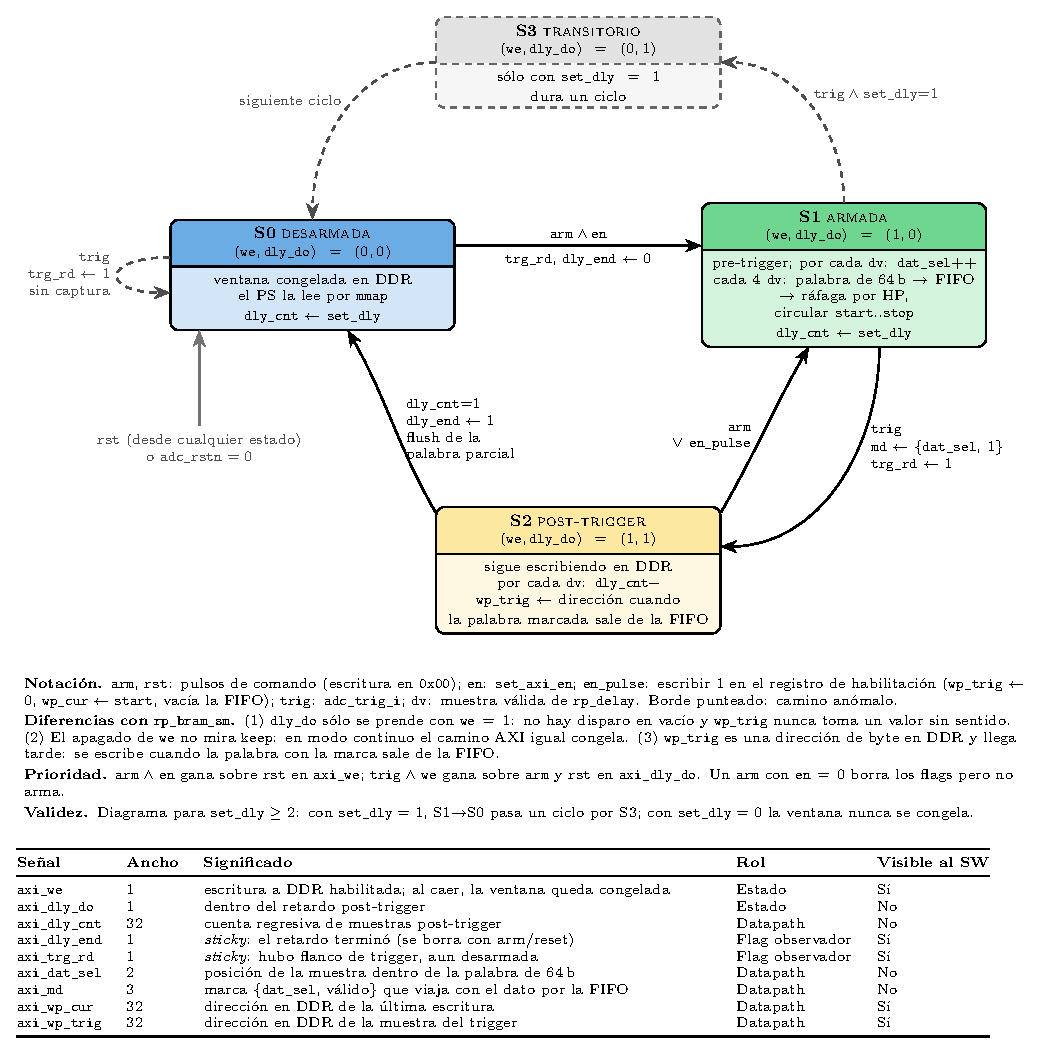
\includegraphics[width=\textwidth]{fsm_rp_axi_sm.pdf}
%
\documentclass[border=0pt,tikz]{standalone}
\usepackage[utf8]{inputenc}
\usepackage[T1]{fontenc}
\usepackage{lmodern}
\usepackage{amsmath}
\usepackage{booktabs}
\usetikzlibrary{arrows.meta,positioning,calc,shapes.multipart,quotes,backgrounds}

% ---------------------------------------------------------------- colores ---
\definecolor{azul}{RGB}{108,172,228}
\definecolor{verde}{RGB}{110,214,142}
\definecolor{amarillo}{RGB}{252,232,160}
\definecolor{grisr}{RGB}{226,226,226}

% ---------------------------------------------------------------- estilos ---
\tikzset{
  >={Stealth[length=2.6mm,width=2mm]},
  estado/.style = {
    rectangle split, rectangle split parts=2, rounded corners=4pt,
    draw=black, line width=0.7pt, align=center, text width=4.6cm,
    inner sep=3pt, font=\footnotesize,
    rectangle split part fill={#1, #1!30},
  },
  anomalo/.style = {estado=grisr, dashed, draw=black!60},
  trans/.style   = {->, line width=0.8pt},
  global/.style  = {->, line width=0.8pt, black!55},
  guarda/.style  = {font=\scriptsize, align=center, fill=white, inner sep=1.5pt},
}

% nombres de señales
\newcommand{\s}[1]{\texttt{#1}}
% encabezado de estado: nombre y codificación (axi_we, axi_dly_do)
\newcommand{\cab}[3]{\textbf{#1}\;\textsc{#2}\\[-1pt]{\scriptsize$(\s{we},\s{dly\_do}) = (#3)$}}

\begin{document}
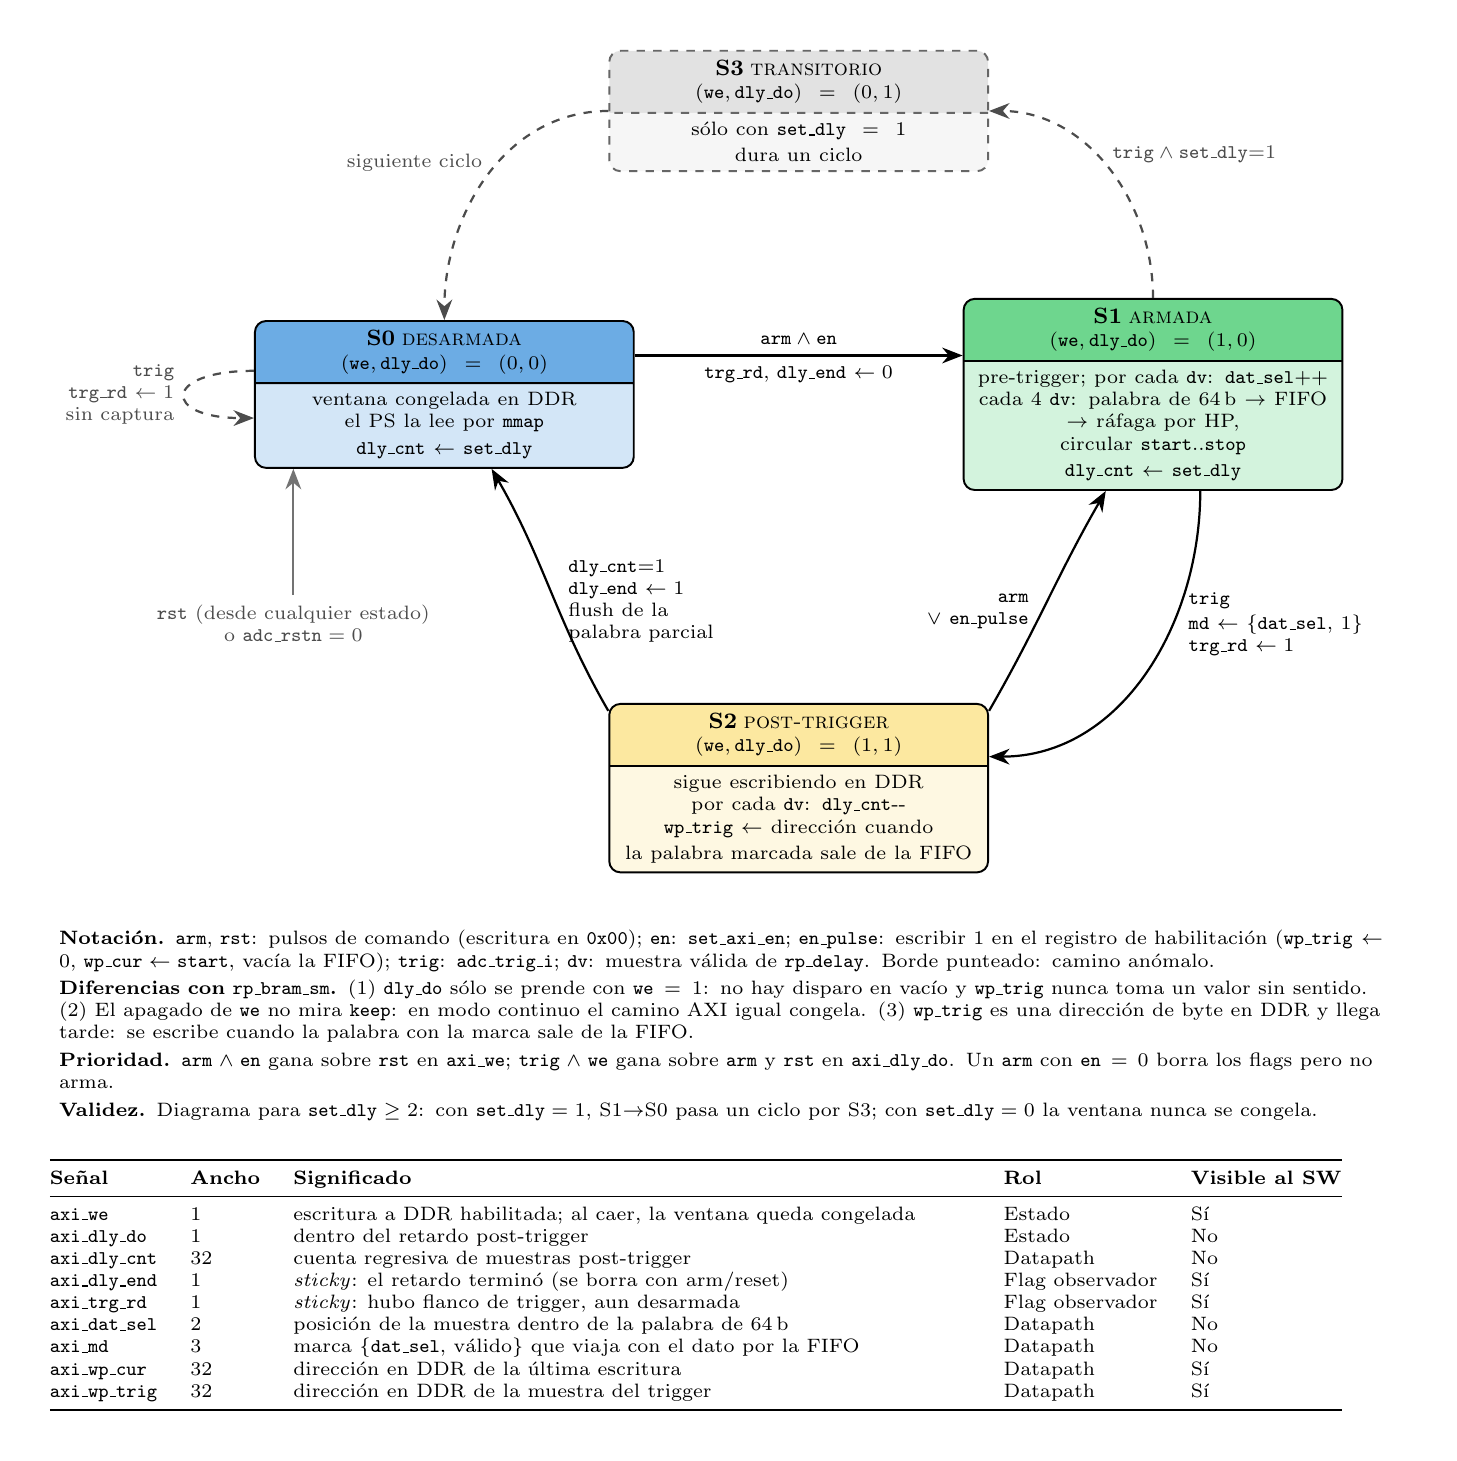
\begin{tikzpicture}[node distance=2cm, show background rectangle, inner frame sep=8pt,
  background rectangle/.style={fill=white, draw=none}]

% ===================================================================== estados
\node[estado=azul] (S0) at (0,0) {
  \cab{S0}{desarmada}{0,0}
  \nodepart{two}\scriptsize ventana congelada en DDR\\
  el PS la lee por \s{mmap}\\
  \s{dly\_cnt} $\leftarrow$ \s{set\_dly}
};

\node[estado=verde] (S1) at (9,0) {
  \cab{S1}{armada}{1,0}
  \nodepart{two}\scriptsize pre-trigger; por cada \s{dv}: \s{dat\_sel}{+}{+}\\
  cada 4 \s{dv}: palabra de 64\,b $\to$ FIFO\\
  $\to$ ráfaga por HP, circular \s{start}..\s{stop}\\
  \s{dly\_cnt} $\leftarrow$ \s{set\_dly}
};

\node[estado=amarillo] (S2) at (4.5,-5) {
  \cab{S2}{post-trigger}{1,1}
  \nodepart{two}\scriptsize sigue escribiendo en DDR\\
  por cada \s{dv}: \s{dly\_cnt}{-}{-}\\
  \s{wp\_trig} $\leftarrow$ dirección cuando\\
  la palabra marcada sale de la FIFO
};

\node[anomalo] (S3) at (4.5,3.6) {
  \cab{S3}{transitorio}{0,1}
  \nodepart{two}\scriptsize sólo con \s{set\_dly}${}=1$\\
  dura un ciclo
};

% ============================================================ reset global ===
\coordinate (rst) at ($(S0.south west)+(0.5,-1.6)$);
\draw[global] (rst) node[below, font=\scriptsize, align=center, black!70]
  {\s{rst} (desde cualquier estado)\\ o \s{adc\_rstn}${}=0$}
  -- (rst |- S0.south);

% ============================================================ transiciones ===
% S0 -> S1 : armar, sólo si el camino AXI está habilitado
\draw[trans] (S0.text split east |- S0.north east) ++(0,-0.45) coordinate (a0)
  (a0) -- (a0 -| S1.west)
  node[guarda, midway, above=2pt, fill=none] {$\s{arm} \wedge \s{en}$}
  node[guarda, midway, below=2pt, fill=none]
  {\s{trg\_rd}, \s{dly\_end} $\leftarrow 0$};

% S1 -> S2 : trigger válido
\draw[trans] ([xshift=6mm]S1.south) to[out=-90, in=0]
  node[guarda, pos=0.35, right=4pt, fill=none, align=left]
  {\s{trig}\\[1pt] \s{md} $\leftarrow$ \{\s{dat\_sel}, 1\}\\ \s{trg\_rd} $\leftarrow 1$}
  ([yshift=4mm]S2.east);

% S2 -> S1 : re-armado o rehabilitación
\draw[trans] ([yshift=-1mm]S2.north east) to[out=60, in=-120]
  node[guarda, pos=0.45, left=3pt, fill=none, align=right]
  {\s{arm}\\ $\vee\ \s{en\_pulse}$}
  ([xshift=-6mm]S1.south);

% S2 -> S0 : fin del post-trigger, congela (no mira keep)
\draw[trans] ([yshift=-1mm]S2.north west) to[out=120, in=-60]
  node[guarda, pos=0.45, right=3pt, fill=none, align=left]
  {$\s{dly\_cnt}{=}1$\\ \s{dly\_end} $\leftarrow 1$\\ flush de la\\ palabra parcial}
  ([xshift=6mm]S0.south);

% S0 -> S0 : trigger con la FSM desarmada, sin captura
\draw[trans, dashed, black!70] (S0.west) ++(0,0.3) coordinate (l0)
  to[out=180, in=180, looseness=5]
  node[guarda, left=2pt, fill=none, align=right]
  {\s{trig}\\ \s{trg\_rd} $\leftarrow 1$\\ sin captura}
  ($(S0.west)+(0,-0.3)$);

% S1 -> S3 -> S0 : set_dly = 1
\draw[trans, dashed, black!70] (S1.north) to[out=90, in=0]
  node[guarda, pos=0.5, above right=0pt, fill=none] {$\s{trig} \wedge \s{set\_dly}{=}1$}
  (S3.east);
\draw[trans, dashed, black!70] (S3.west) to[out=180, in=90]
  node[guarda, pos=0.5, above left=0pt, fill=none] {siguiente ciclo}
  (S0.north);

% ================================================================= leyenda ===
\node[font=\scriptsize, align=left, anchor=north west, text width=17cm]
  (ley) at ($(S0.west |- S2.south)+(-2.6,-0.6)$) {%
  \textbf{Notación.} \s{arm}, \s{rst}: pulsos de comando (escritura en \s{0x00});
  \s{en}: \s{set\_axi\_en}; \s{en\_pulse}: escribir 1 en el registro de habilitación
  (\s{wp\_trig}${}\leftarrow 0$, \s{wp\_cur}${}\leftarrow{}$\s{start}, vacía la FIFO);
  \s{trig}: \s{adc\_trig\_i}; \s{dv}: muestra válida de \s{rp\_delay}.
  Borde punteado: camino anómalo.\\[2pt]
  \textbf{Diferencias con \s{rp\_bram\_sm}.}
  (1) \s{dly\_do} sólo se prende con \s{we}${}=1$: no hay disparo en vacío y
  \s{wp\_trig} nunca toma un valor sin sentido.
  (2) El apagado de \s{we} no mira \s{keep}: en modo continuo el camino AXI
  igual congela.
  (3) \s{wp\_trig} es una dirección de byte en DDR y llega tarde: se escribe
  cuando la palabra con la marca sale de la FIFO.\\[2pt]
  \textbf{Prioridad.} $\s{arm}\wedge\s{en}$ gana sobre \s{rst} en \s{axi\_we};
  $\s{trig}\wedge\s{we}$ gana sobre \s{arm} y \s{rst} en \s{axi\_dly\_do}.
  Un \s{arm} con \s{en}${}=0$ borra los flags pero no arma.\\[2pt]
  \textbf{Validez.} Diagrama para \s{set\_dly}${}\ge 2$: con \s{set\_dly}${}=1$,
  S1$\to$S0 pasa un ciclo por S3; con \s{set\_dly}${}=0$ la ventana nunca se congela.%
};

% ================================================================ banderas ===
\node[font=\scriptsize, anchor=north west, inner sep=0pt]
  at ($(ley.south west)+(0,-0.35)$) {%
  \begin{tabular}{@{}llp{8.6cm}ll@{}}
    \toprule
    \textbf{Señal} & \textbf{Ancho} & \textbf{Significado} & \textbf{Rol} & \textbf{Visible al SW} \\
    \midrule
    \s{axi\_we}      & 1  & escritura a DDR habilitada; al caer, la ventana queda congelada & Estado          & Sí \\
    \s{axi\_dly\_do} & 1  & dentro del retardo post-trigger                                 & Estado          & No \\
    \s{axi\_dly\_cnt}& 32 & cuenta regresiva de muestras post-trigger                       & Datapath        & No \\
    \s{axi\_dly\_end}& 1  & \emph{sticky}: el retardo terminó (se borra con arm/reset)      & Flag observador & Sí \\
    \s{axi\_trg\_rd} & 1  & \emph{sticky}: hubo flanco de trigger, aun desarmada            & Flag observador & Sí \\
    \s{axi\_dat\_sel}& 2  & posición de la muestra dentro de la palabra de 64\,b            & Datapath        & No \\
    \s{axi\_md}      & 3  & marca \{\s{dat\_sel}, válido\} que viaja con el dato por la FIFO & Datapath       & No \\
    \s{axi\_wp\_cur} & 32 & dirección en DDR de la última escritura                         & Datapath        & Sí \\
    \s{axi\_wp\_trig}& 32 & dirección en DDR de la muestra del trigger                      & Datapath        & Sí \\
    \bottomrule
  \end{tabular}%
};

\end{tikzpicture}
\end{document}
